% Options for packages loaded elsewhere
\PassOptionsToPackage{unicode}{hyperref}
\PassOptionsToPackage{hyphens}{url}
%
\documentclass[
]{book}
\usepackage{amsmath,amssymb}
\usepackage{lmodern}
\usepackage{ifxetex,ifluatex}
\ifnum 0\ifxetex 1\fi\ifluatex 1\fi=0 % if pdftex
  \usepackage[T1]{fontenc}
  \usepackage[utf8]{inputenc}
  \usepackage{textcomp} % provide euro and other symbols
\else % if luatex or xetex
  \usepackage{unicode-math}
  \defaultfontfeatures{Scale=MatchLowercase}
  \defaultfontfeatures[\rmfamily]{Ligatures=TeX,Scale=1}
\fi
% Use upquote if available, for straight quotes in verbatim environments
\IfFileExists{upquote.sty}{\usepackage{upquote}}{}
\IfFileExists{microtype.sty}{% use microtype if available
  \usepackage[]{microtype}
  \UseMicrotypeSet[protrusion]{basicmath} % disable protrusion for tt fonts
}{}
\makeatletter
\@ifundefined{KOMAClassName}{% if non-KOMA class
  \IfFileExists{parskip.sty}{%
    \usepackage{parskip}
  }{% else
    \setlength{\parindent}{0pt}
    \setlength{\parskip}{6pt plus 2pt minus 1pt}}
}{% if KOMA class
  \KOMAoptions{parskip=half}}
\makeatother
\usepackage{xcolor}
\IfFileExists{xurl.sty}{\usepackage{xurl}}{} % add URL line breaks if available
\IfFileExists{bookmark.sty}{\usepackage{bookmark}}{\usepackage{hyperref}}
\hypersetup{
  pdftitle={OTESSA 2022 Program},
  pdfauthor={Open Technology in Education, Society, and Scholarship Association},
  hidelinks,
  pdfcreator={LaTeX via pandoc}}
\urlstyle{same} % disable monospaced font for URLs
\usepackage{longtable,booktabs,array}
\usepackage{calc} % for calculating minipage widths
% Correct order of tables after \paragraph or \subparagraph
\usepackage{etoolbox}
\makeatletter
\patchcmd\longtable{\par}{\if@noskipsec\mbox{}\fi\par}{}{}
\makeatother
% Allow footnotes in longtable head/foot
\IfFileExists{footnotehyper.sty}{\usepackage{footnotehyper}}{\usepackage{footnote}}
\makesavenoteenv{longtable}
\usepackage{graphicx}
\makeatletter
\def\maxwidth{\ifdim\Gin@nat@width>\linewidth\linewidth\else\Gin@nat@width\fi}
\def\maxheight{\ifdim\Gin@nat@height>\textheight\textheight\else\Gin@nat@height\fi}
\makeatother
% Scale images if necessary, so that they will not overflow the page
% margins by default, and it is still possible to overwrite the defaults
% using explicit options in \includegraphics[width, height, ...]{}
\setkeys{Gin}{width=\maxwidth,height=\maxheight,keepaspectratio}
% Set default figure placement to htbp
\makeatletter
\def\fps@figure{htbp}
\makeatother
\setlength{\emergencystretch}{3em} % prevent overfull lines
\providecommand{\tightlist}{%
  \setlength{\itemsep}{0pt}\setlength{\parskip}{0pt}}
\setcounter{secnumdepth}{5}
\usepackage{booktabs}
\usepackage{amsthm}
\makeatletter
\def\thm@space@setup{%
  \thm@preskip=8pt plus 2pt minus 4pt
  \thm@postskip=\thm@preskip
}
\makeatother
\ifluatex
  \usepackage{selnolig}  % disable illegal ligatures
\fi
\usepackage[]{natbib}
\bibliographystyle{apalike}

\title{OTESSA 2022 Program}
\author{Open Technology in Education, Society, and Scholarship Association}
\date{Last updated 2022-04-13}

\begin{document}
\maketitle

{
\setcounter{tocdepth}{1}
\tableofcontents
}
\hypertarget{welcome}{%
\chapter*{Welcome}\label{welcome}}
\addcontentsline{toc}{chapter}{Welcome}

\begin{todo}
\hypertarget{note}{%
\paragraph*{✨ Note}\label{note}}
\addcontentsline{toc}{paragraph}{✨ Note}

\textbf{\emph{All times are in Eastern Time (Canada)}}
\end{todo}

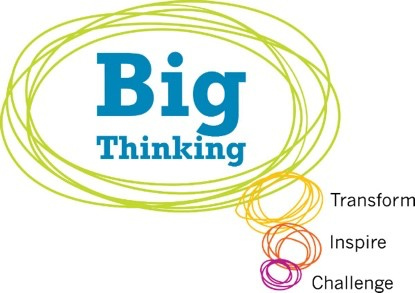
\includegraphics{assets/media/image2.jpeg}

All OTESSA Participants can attend the \href{https://www.federationhss.ca/en/congress/congress-2022/open-programming}{Congress ``Big Thinking'' lecture series}. These take place each day of the conference. Congress has ``\href{https://www.federationhss.ca/en/congress/congress-2022/calendar-open-events}{open events}'' available as well (open to registrants across association conferences at Congress as well as those who hold community passes).

All OTESSA Registrants can also attend conference sessions offered by the \href{https://csse-scee.ca/}{Canadian Association for the Study of Education (CSSE)}, \href{https://csshe-scees.ca/}{Canadian Association for the Study of Higher Education (CSSHE)}, \href{https://www.calj-acrs.ca/}{Canadian Association of Learned Journals (CALJ)}, and \href{https://www.casae-aceea.ca/}{Canadian Association for the Study of Adult Education (CASAE)} as we have reciprocity agreements in place.

Please note that presenters must register in each conference in which they are presenting.

\hypertarget{keynotes}{%
\chapter*{Keynotes}\label{keynotes}}
\addcontentsline{toc}{chapter}{Keynotes}

\hypertarget{martin-weller}{%
\section*{Martin Weller}\label{martin-weller}}
\addcontentsline{toc}{section}{Martin Weller}

\begin{reflect}
\hypertarget{metaphors-of-edtech}{%
\subsubsection{Metaphors of EdTech}\label{metaphors-of-edtech}}

In this talk, I will explore why metaphors are both a useful and
potentially misleading way of thinking about educational technology. A
number of metaphors will be proposed and analysed which demonstrate how
metaphors can shape our thinking and help us view educational technology
from different perspectives. The Covid pandemic saw nearly all education
institutions engaging in an online pivot, which usually involved online
versions of existing practices, such as lectures. As we seek to build on
this experience and offer a richer online experience it has become
evident that the face-to-face lecture has become a dominant model that
many struggle to see past. This talk will examine how different
metaphors can help us approach educational technology.
\end{reflect}

\hypertarget{sherri-spelic}{%
\section*{Sherri Spelic}\label{sherri-spelic}}
\addcontentsline{toc}{section}{Sherri Spelic}

\begin{reflect}
\hypertarget{hide-and-seek-on-kids-power-and-resistance-in-education}{%
\subsubsection{Hide and Seek: On Kids, Power, and Resistance in
Education}\label{hide-and-seek-on-kids-power-and-resistance-in-education}}

I want to explore what happens when the learners in our care resist our
offer of help, expertise, and teaching. How do we make sense of students
applying refusal skills in the classroom? Rather than provide answers I
will draw on student statements about the possibility and significance
of saying ``no'' at school and use these to probe our understanding and
appreciation of power in students' hands and voices. We'll also pose the
question: to what degree do our pedagogies leave space for negotiation
and power sharing? And where does this show itself in practice?
\end{reflect}

\hypertarget{maha-bali}{%
\section*{Maha Bali}\label{maha-bali}}
\addcontentsline{toc}{section}{Maha Bali}

\begin{reflect}
\hypertarget{outside-in-openness-as-subversion}{%
\subsubsection{Outside-In: Openness as
Subversion}\label{outside-in-openness-as-subversion}}

We often talk about how open education expands access, supports
knowledge sharing, and potentially enhances the quality of education. We
also critique open education for sometimes reproducing inequalities
despite promising to promote social justice.\\
But what about the ways in which ``openness'' removes/destroys barriers
within us? In what ways does openness empower us from the outside-in?
When does openness influence critical change and when might it fail to
do so?\\
In this interactive session, we will explore some of the things openness
makes possible that are often not possible within the walls of
institutions, and which can end up challenging and subverting injustice.
\end{reflect}

\hypertarget{brenna-clarke-gray}{%
\section*{Brenna Clarke Gray}\label{brenna-clarke-gray}}
\addcontentsline{toc}{section}{Brenna Clarke Gray}

\begin{reflect}
\hypertarget{things-unsaid-exploring-the-margins-and-limits-of-open}{%
\subsubsection{Things Unsaid: Exploring the Margins and Limits of
Open}\label{things-unsaid-exploring-the-margins-and-limits-of-open}}

Open is not an unambiguous good, a panacea, or accessible to everyone.
But maybe it could be more of all of those things if, as a community, we
could talk more openly about open's borders and limitations. What does
it mean to say we are a community of open educators? What is the edge of
open-ness, and how do we account for its definition? What --- and whose
--- truths remain unsaid or unspoken even in communities that define
themselves as open? And who is safe to choose open? Offering an
autoethnography of pregnancy loss set against the backdrop of the
pandemic university as a place to start this exploration, this talk
looks to chart the margins and limits of open and to ask about the
benefits of expanding the scope and possibilities of openness in our
institutions. It invites all of us to imagine a more perfect open, or at
least to consider how more of us can be supported to speak our things
unsaid.
\end{reflect}

\hypertarget{monday-may-16-2022}{%
\chapter{Monday, May 16, 2022}\label{monday-may-16-2022}}

\hypertarget{legend}{%
\subsection*{Legend}\label{legend}}
\addcontentsline{toc}{subsection}{Legend}

\begin{wp}
\hypertarget{invited-speaker}{%
\paragraph{Invited Speaker}\label{invited-speaker}}
\end{wp}

\begin{reflect}
\hypertarget{keynote}{%
\paragraph{Keynote}\label{keynote}}
\end{reflect}

\begin{secondary}
\hypertarget{presentation}{%
\paragraph{Presentation}\label{presentation}}
\end{secondary}

\begin{center}\rule{0.5\linewidth}{0.5pt}\end{center}

\hypertarget{welcome-desk-open-1030---1230}{%
\section*{Welcome Desk Open (10:30 - 12:30)}\label{welcome-desk-open-1030---1230}}
\addcontentsline{toc}{section}{Welcome Desk Open (10:30 - 12:30)}

\hypertarget{conference-welcome-and-keynote-1100---1230}{%
\section*{Conference Welcome and Keynote (11:00 - 12:30)}\label{conference-welcome-and-keynote-1100---1230}}
\addcontentsline{toc}{section}{Conference Welcome and Keynote (11:00 - 12:30)}

\begin{reflect}
\hypertarget{metaphors-of-ed-tech}{%
\paragraph{Metaphors of Ed Tech}\label{metaphors-of-ed-tech}}

\emph{Martin Weller}\\
\href{https://otessa.github.io/2022/keynotes-intro.html\#metaphors-of-edtech}{Abstract}
\end{reflect}

\hypertarget{break-1230---100}{%
\section*{Break (12:30 - 1:00)}\label{break-1230---100}}
\addcontentsline{toc}{section}{Break (12:30 - 1:00)}

\hypertarget{parallel-session-1-100-145}{%
\section*{Parallel Session 1 (1:00 -- 1:45)}\label{parallel-session-1-100-145}}
\addcontentsline{toc}{section}{Parallel Session 1 (1:00 -- 1:45)}

Invited Speaker Options

\hypertarget{parallel-session-1.1}{%
\subsection*{Parallel Session 1.1}\label{parallel-session-1.1}}
\addcontentsline{toc}{subsection}{Parallel Session 1.1}

\begin{wp}
\hypertarget{embracing-the-middle}{%
\paragraph{\texorpdfstring{\textbf{Embracing the
Middle}}{Embracing the Middle}}\label{embracing-the-middle}}

\emph{Jess Mitchell}
\end{wp}

\hypertarget{parallel-session-1.2}{%
\subsection*{Parallel Session 1.2}\label{parallel-session-1.2}}
\addcontentsline{toc}{subsection}{Parallel Session 1.2}

\begin{wp}
\hypertarget{one-for-all-all-for-one-to-support-and-enable-our-learning-societies}{%
\paragraph{\texorpdfstring{\textbf{One for All, All for One, to Support
and Enable Our Learning
Societies}}{One for All, All for One, to Support and Enable Our Learning Societies}}\label{one-for-all-all-for-one-to-support-and-enable-our-learning-societies}}

\emph{Nadia Naffi}
\end{wp}

\hypertarget{break-145-215}{%
\section*{Break (1:45 -- 2:15)}\label{break-145-215}}
\addcontentsline{toc}{section}{Break (1:45 -- 2:15)}

\hypertarget{parallel-session-2-215-345}{%
\section*{Parallel Session 2 (2:15 -- 3:45)}\label{parallel-session-2-215-345}}
\addcontentsline{toc}{section}{Parallel Session 2 (2:15 -- 3:45)}

\hypertarget{parallel-session-2.1---wildcard-indigenous-language-revival-k12-truth-reconciliation}{%
\subsection*{Parallel Session 2.1 - WILDCARD: Indigenous Language Revival \& K12 Truth \& Reconciliation}\label{parallel-session-2.1---wildcard-indigenous-language-revival-k12-truth-reconciliation}}
\addcontentsline{toc}{subsection}{Parallel Session 2.1 - WILDCARD: Indigenous Language Revival \& K12 Truth \& Reconciliation}

\begin{secondary}
\hypertarget{section}{%
\paragraph{2:15-2:45}\label{section}}

\textbf{Elders' Conversations: Perspectives on leveraging digital
technology in language revival (Research-Oriented)}

\emph{Melissa Bishop}
\end{secondary}

\begin{secondary}
\hypertarget{section}{%
\paragraph*{2:45-3:45}\label{section}}
\addcontentsline{toc}{paragraph}{2:45-3:45}

\textbf{Truth and Reconciliation Through Inquiry-based Collaborative
Learning (Practice-Oriented)}

\emph{Deirdre Houghton (Nechako Lakes School District \& University of
Victoria), Gary Soles (Nechako Lakes School District \& University of
Victoria), Andrew Vogelsang (Nechako Lakes School District \& University
of Victoria), Valerie Irvine (University of Victoria)}
\end{secondary}

\hypertarget{parallel-session-2.2-sustaining-positive-change-pse-ethics-pse-scholarship}{%
\subsection*{Parallel Session 2.2 -- Sustaining Positive Change: PSE Ethics \& PSE Scholarship}\label{parallel-session-2.2-sustaining-positive-change-pse-ethics-pse-scholarship}}
\addcontentsline{toc}{subsection}{Parallel Session 2.2 -- Sustaining Positive Change: PSE Ethics \& PSE Scholarship}

\begin{secondary}
\hypertarget{section}{%
\paragraph*{2:15-2:45}\label{section}}
\addcontentsline{toc}{paragraph}{2:15-2:45}

\textbf{Surveillance in the System: Data as Critical Change in Higher
Education (Research-Oriented)}

\emph{Bonnie Stewart (University of Windsor), Samatha Szcyrek
(University of Windsor)}
\end{secondary}

\begin{secondary}
\hypertarget{section}{%
\paragraph*{2:45-3:45}\label{section}}
\addcontentsline{toc}{paragraph}{2:45-3:45}

\textbf{Cognification in Education in Light of the Fourth Industrial
Revolution (Research-Oriented)}

\emph{Vivekanandan Kumar (Athabasca University), Mohamed Ally (Athabasca
University), Avgoustos Tsinakos (International Hellenic University),
Muhammad Helmi Norman (Universiti Kebangsaan Malaysia)}
\end{secondary}

\hypertarget{parallel-session-2.3-transitions-of-online-learning-and-teaching-e-texts-oer}{%
\subsection*{Parallel Session 2.3 -- Transitions of Online Learning and Teaching: E-Texts / OER}\label{parallel-session-2.3-transitions-of-online-learning-and-teaching-e-texts-oer}}
\addcontentsline{toc}{subsection}{Parallel Session 2.3 -- Transitions of Online Learning and Teaching: E-Texts / OER}

\begin{secondary}
\hypertarget{section}{%
\paragraph*{2:15-2:45}\label{section}}
\addcontentsline{toc}{paragraph}{2:15-2:45}

\textbf{Investigating the effects of computer-generated contextual
landmarks on short-term recall of e-texts (Research-Oriented)}

\emph{Jon Dron, Rory McGreal, Vive Kumar, Jennifer Davies (Athabasca
University)}
\end{secondary}

\begin{secondary}
\hypertarget{section}{%
\paragraph*{2:45-3:45}\label{section}}
\addcontentsline{toc}{paragraph}{2:45-3:45}

\textbf{Community-Led Infrastructures for Open Access Books: A
Sustainable Model and Platform (Practice-Oriented)}

\emph{Judith Fathallah (Lancaster University), Martin Eve (University of
London, Tom Grady (University of London)}
\end{secondary}

\hypertarget{parallel-session-2.4}{%
\subsection*{Parallel Session 2.4}\label{parallel-session-2.4}}
\addcontentsline{toc}{subsection}{Parallel Session 2.4}

\begin{secondary}
\hypertarget{time}{%
\paragraph{\texorpdfstring{\texttt{TIME}}{TIME}}\label{time}}

\textbf{Flexible approaches to learning: Bridging inclusive/exclusive
spaces through open educational practice (Practice-Oriented)}

\emph{Michelle Harrison (Thompson Rivers University)}
\end{secondary}

\begin{secondary}
\hypertarget{time}{%
\paragraph{\texorpdfstring{\texttt{TIME}}{TIME}}\label{time}}

\textbf{Warp and Weft: Weaving and Open Dissertation
(Practice-Oriented)}

\emph{Helen Dewaard (Lakehead University \& University of British
Columbia), Leo Havemann (University College London), Verena Roberts
(University of Calgary \& Thompson Rivers University)}
\end{secondary}

\begin{secondary}
\hypertarget{time}{%
\paragraph{\texorpdfstring{\texttt{TIME}}{TIME}}\label{time}}

\textbf{Incorporating Open Educational Pedagogies and Co-mentorship
Practices in Graduate Education (Research-Oriented)}

\emph{Cindy Ives (Athabasca University)}
\end{secondary}

\begin{secondary}
\hypertarget{time}{%
\paragraph{\texorpdfstring{\texttt{TIME}}{TIME}}\label{time}}

\textbf{Critical reflection: How can open reflexive frameworks redefine
academic practices? (Practice-Oriented)}

\emph{Helen DeWaard (Lakehead University \& University of British
Columbia), Shauna Burnie (Lakehead University)}
\end{secondary}

\hypertarget{parallel-session-2.5}{%
\subsection*{Parallel Session 2.5}\label{parallel-session-2.5}}
\addcontentsline{toc}{subsection}{Parallel Session 2.5}

\begin{secondary}
\hypertarget{sustaining-positive-change-pse-open}{%
\paragraph*{2:15-2:45 -- Sustaining Positive Change -- PSE
Open}\label{sustaining-positive-change-pse-open}}
\addcontentsline{toc}{paragraph}{2:15-2:45 -- Sustaining Positive Change
-- PSE Open}

\textbf{Open educational practice and research resources created by
students, for students (Practice-Oriented)}

\emph{Marie Bartlett \& Students (Thompson Rivers University)}
\end{secondary}

\begin{secondary}
\hypertarget{transitions-of-online-learning-and-teaching-pse-online}{%
\paragraph*{2:45-3:45: -- Transitions of Online Learning and Teaching --
PSE
Online}\label{transitions-of-online-learning-and-teaching-pse-online}}
\addcontentsline{toc}{paragraph}{2:45-3:45: -- Transitions of Online
Learning and Teaching -- PSE Online}

\textbf{Building digital fluency skills during the rapid transition to
online and hybrid teaching through open access with the Ontario Extend
program (Practice-Oriented)}

\emph{Alissa Bigelow (eCampusOntario)}
\end{secondary}

\hypertarget{break-345-400}{%
\section*{Break (3:45 -- 4:00)}\label{break-345-400}}
\addcontentsline{toc}{section}{Break (3:45 -- 4:00)}

\hypertarget{social-session-400-430}{%
\section*{Social Session (4:00 -- 4:30)}\label{social-session-400-430}}
\addcontentsline{toc}{section}{Social Session (4:00 -- 4:30)}

\begin{gh}
\hypertarget{social-gurdeep-pandher-of-the-yukon}{%
\paragraph*{Social: Gurdeep Pandher of the
Yukon}\label{social-gurdeep-pandher-of-the-yukon}}
\addcontentsline{toc}{paragraph}{Social: Gurdeep Pandher of the Yukon}

\textbf{Bhangra dance class}
\end{gh}

\hypertarget{parallel-session-3-430-530}{%
\section*{Parallel Session 3 (4:30 -- 5:30)}\label{parallel-session-3-430-530}}
\addcontentsline{toc}{section}{Parallel Session 3 (4:30 -- 5:30)}

\hypertarget{parallel-session-3.1-sustaining-positive-change-k12-greentech}{%
\subsection*{Parallel Session 3.1 -- Sustaining Positive Change: K12, GreenTech}\label{parallel-session-3.1-sustaining-positive-change-k12-greentech}}
\addcontentsline{toc}{subsection}{Parallel Session 3.1 -- Sustaining Positive Change: K12, GreenTech}

\begin{secondary}
\hypertarget{time}{%
\paragraph{\texorpdfstring{\texttt{Time}}{Time}}\label{time}}

\textbf{Improving environmental sustainability by using public school
systems as centers of green energy production and conservation:
Approaches to offsetting the cost of increased technology use and
associated pollution (Practice-Oriented)}

\emph{Scott Warren, Scott Moran, Kristen McGuffin (University of North
Texas)}
\end{secondary}

\hypertarget{parallel-session-3.2-sustaining-positive-change-pse-open}{%
\subsection*{Parallel Session 3.2 -- Sustaining Positive Change -- PSE Open}\label{parallel-session-3.2-sustaining-positive-change-pse-open}}
\addcontentsline{toc}{subsection}{Parallel Session 3.2 -- Sustaining Positive Change -- PSE Open}

\begin{secondary}
\hypertarget{time}{%
\paragraph{\texorpdfstring{\texttt{TIME}}{TIME}}\label{time}}

\textbf{Sustaining Complexity: Why Higher Education Should Avoid
TechnoSolutionism (Practice-Oriented)}

\emph{Jim Luke (Lansing Community College), Bonnie Stewart (University
of Windsor)}
\end{secondary}

\hypertarget{parallel-session-3.3-addressing-the-new-inequities-critical-edtech}{%
\subsection*{Parallel Session 3.3 -- Addressing the New Inequities: Critical EdTech}\label{parallel-session-3.3-addressing-the-new-inequities-critical-edtech}}
\addcontentsline{toc}{subsection}{Parallel Session 3.3 -- Addressing the New Inequities: Critical EdTech}

\begin{secondary}
\hypertarget{time}{%
\paragraph{\texorpdfstring{\texttt{time}}{time}}\label{time}}

\textbf{Rejecting the ready-made future: Reimagining technologies from
and for the classroom (Research-Oriented)}

\emph{Esteban Morales, Rachel Horst (University of British Columbia)}
\end{secondary}

\hypertarget{parallel-session-3.4-addressing-the-new-inequities-open}{%
\subsection*{Parallel Session 3.4 -- Addressing the New Inequities: Open}\label{parallel-session-3.4-addressing-the-new-inequities-open}}
\addcontentsline{toc}{subsection}{Parallel Session 3.4 -- Addressing the New Inequities: Open}

\begin{secondary}
\hypertarget{time}{%
\paragraph{\texorpdfstring{\texttt{TIME}}{TIME}}\label{time}}

\textbf{Open Educational Practices (OEP): Critical Policy Analysis in
the Canadian Post-Secondary Education Context (Research-Oriented)}

\emph{Mara Bordignon (University of Western Ontario)}
\end{secondary}

\hypertarget{parallel-session-3.5-transitions-of-online-learning-and-teaching-online-society}{%
\subsection*{Parallel Session 3.5 -- Transitions of Online Learning and Teaching -- Online \& Society}\label{parallel-session-3.5-transitions-of-online-learning-and-teaching-online-society}}
\addcontentsline{toc}{subsection}{Parallel Session 3.5 -- Transitions of Online Learning and Teaching -- Online \& Society}

\begin{secondary}
\hypertarget{time}{%
\paragraph{\texorpdfstring{\texttt{TIME}}{TIME}}\label{time}}

\textbf{Online or Remote Learning and Mental Health (Research-Oriented)}

\emph{Stephanie Moore (University of New Mexico), Michael Barbour (Touro
University California), George Veletsianos (Royal Roads University)}
\end{secondary}

\hypertarget{break-530---600}{%
\section*{Break (5:30 - 6:00)}\label{break-530---600}}
\addcontentsline{toc}{section}{Break (5:30 - 6:00)}

\hypertarget{parallel-session-4-600---645}{%
\section*{Parallel Session 4 (6:00 - 6:45)}\label{parallel-session-4-600---645}}
\addcontentsline{toc}{section}{Parallel Session 4 (6:00 - 6:45)}

Invited Speakers

\hypertarget{parallel-session-4.1}{%
\subsection*{Parallel Session 4.1}\label{parallel-session-4.1}}
\addcontentsline{toc}{subsection}{Parallel Session 4.1}

\begin{reflect}
\hypertarget{land-use-metaphor-in-scholarly-communication-a-brief-inventory-and-inspection}{%
\paragraph*{Land-use Metaphor in Scholarly Communication: A Brief
Inventory and
Inspection}\label{land-use-metaphor-in-scholarly-communication-a-brief-inventory-and-inspection}}
\addcontentsline{toc}{paragraph}{Land-use Metaphor in Scholarly
Communication: A Brief Inventory and Inspection}

\emph{AJ Boston}
\end{reflect}

\hypertarget{parallel-session-4.2}{%
\subsection*{Parallel Session 4.2}\label{parallel-session-4.2}}
\addcontentsline{toc}{subsection}{Parallel Session 4.2}

\begin{reflect}
\hypertarget{critical-change-in-online-education---what-we-can-learn-and-not-learn-from-covid-as-a-context}{%
\paragraph*{Critical Change in Online Education - What We Can Learn (And
Not Learn) From COVID as a
Context}\label{critical-change-in-online-education---what-we-can-learn-and-not-learn-from-covid-as-a-context}}
\addcontentsline{toc}{paragraph}{Critical Change in Online Education -
What We Can Learn (And Not Learn) From COVID as a Context}

\emph{Matt Bower}
\end{reflect}

\hypertarget{discussionnetworking-pods-645-700}{%
\section*{Discussion/Networking Pods (6:45 -- 7:00)}\label{discussionnetworking-pods-645-700}}
\addcontentsline{toc}{section}{Discussion/Networking Pods (6:45 -- 7:00)}

\hypertarget{abstracts}{%
\chapter{Abstracts}\label{abstracts}}

\begin{todo}
\hypertarget{note}{%
\paragraph*{✨ Note}\label{note}}
\addcontentsline{toc}{paragraph}{✨ Note}

Abstracts linked in with daily schedule
\end{todo}

  \bibliography{book.bib}

\end{document}
